%%%%%%%%%%%%%%%%%%%%%%%%%%%%%%%%%%%%%%%%%%%%%%%%%%%%%%%%%%%%
%%  This Beamer template was created by Cameron Bracken.
%%  Anyone can freely use or modify it for any purpose
%%  without attribution.
%%
%%  Last Modified: January 9, 2009
%%

\documentclass[xcolor=x11names,compress]{beamer}

%% General document %%%%%%%%%%%%%%%%%%%%%%%%%%%%%%%%%%
\usepackage{graphicx}
\usepackage{tikz}
\usetikzlibrary{decorations.fractals}
%%%%%%%%%%%%%%%%%%%%%%%%%%%%%%%%%%%%%%%%%%%%%%%%%%%%%%


%% Beamer Layout %%%%%%%%%%%%%%%%%%%%%%%%%%%%%%%%%%
\useoutertheme[subsection=false,shadow]{miniframes}
\useinnertheme{default}
\usefonttheme{serif}
\usepackage{palatino}

\setbeamerfont{title like}{shape=\scshape}
\setbeamerfont{frametitle}{shape=\scshape}

\setbeamercolor*{lower separation line head}{bg=DeepSkyBlue4} 
\setbeamercolor*{normal text}{fg=black,bg=white} 
\setbeamercolor*{alerted text}{fg=red} 
\setbeamercolor*{example text}{fg=black} 
\setbeamercolor*{structure}{fg=black} 
 
\setbeamercolor*{palette tertiary}{fg=black,bg=black!10} 
\setbeamercolor*{palette quaternary}{fg=black,bg=black!10} 

\renewcommand{\(}{\begin{columns}}
\renewcommand{\)}{\end{columns}}
\newcommand{\<}[1]{\begin{column}{#1}}
\renewcommand{\>}{\end{column}}
%%%%%%%%%%%%%%%%%%%%%%%%%%%%%%%%%%%%%%%%%%%%%%%%%%




\begin{document}


%%%%%%%%%%%%%%%%%%%%%%%%%%%%%%%%%%%%%%%%%%%%%%%%%%%%%%
%%%%%%%%%%%%%%%%%%%%%%%%%%%%%%%%%%%%%%%%%%%%%%%%%%%%%%
\section{\scshape Index}
\begin{frame}
\title{Contex Stimuli Valence and Age Effects in Time-Based Prospective Memory}
%\subtitle{SUBTITLE}
\author{
	Steven Gonz\'{a}lez Lugo\\ {\tiny Ruth Ferreira Santos-Galdur\'{o}z (orientadora) **\ Marcelo S. Caetano (coorientador)}\\
	{\it Universidade Federal do ABC
	}\\ 
\includegraphics[width=2.8cm]{sigla-abaixo-rgb.png}
}
\date{August 22, 2017}
\titlepage
\end{frame}

%%%%%%%%%%%%%%%%%%%%%%%%%%%%%%%%%%%%%%%%%%%%%%%%%%%%%%
%%%%%%%%%%%%%%%%%%%%%%%%%%%%%%%%%%%%%%%%%%%%%%%%%%%%%%
\begin{frame}
\tableofcontents
\end{frame}

%%%%%%%%%%%%%%%%%%%%%%%%%%%%%%%%%%%%%%%%%%%%%%%%%%%%%%
%%%%%%%%%%%%%%%%%%%%%%%%%%%%%%%%%%%%%%%%%%%%%%%%%%%%%%
\section{\scshape Literature Review}
\subsection{Prospective Memory}
\begin{frame}{What is Prospective Memory?}
\begin{figure}[hbtp]
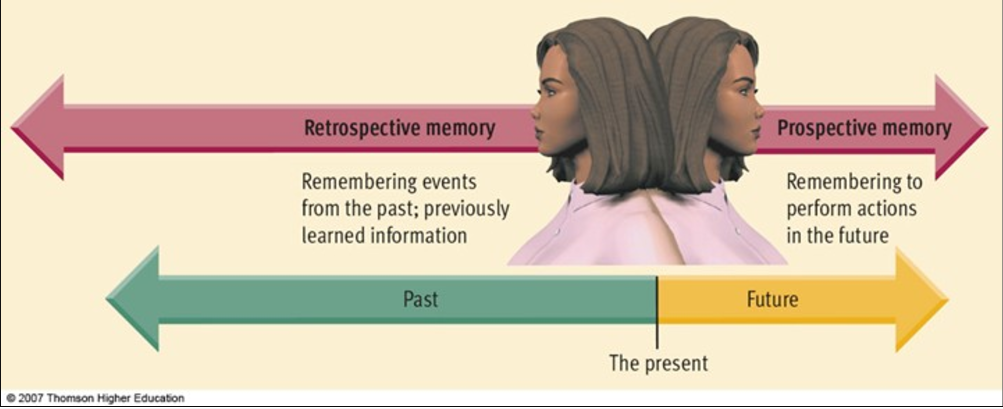
\includegraphics[width=10cm, height=6cm]{INTRO.png}
\centering
\end{figure}


%\begin{itemize}

%\item Retrospective Memory: Memory for people, words, and events experienced in the past.
%\item Prospective memory: memory that involves remembering to carry out intended actions without being instructed to do so.
%\item Time-based prospective memory: A form of prospective memory in which time is the cue indicating that a given action needs to be performed.
%\item Event-based prospective memory: A form of prospective memory in which some event provides the cue to perform a given action.
%\end{itemize}
\end{frame}

%%%%%%%%%%%%%%%%%%%%%%%%%%%%%%%%%%%%%%%%%%%%%%%%%%%%%%
%%%%%%%%%%%%%%%%%%%%%%%%%%%%%%%%%%%%%%%%%%%%%%%%%%%%%%
\subsection{Laboratory Based Prospective Memory Tasks}
\begin{frame}{Laboratory Based Prospective Memory Tasks}
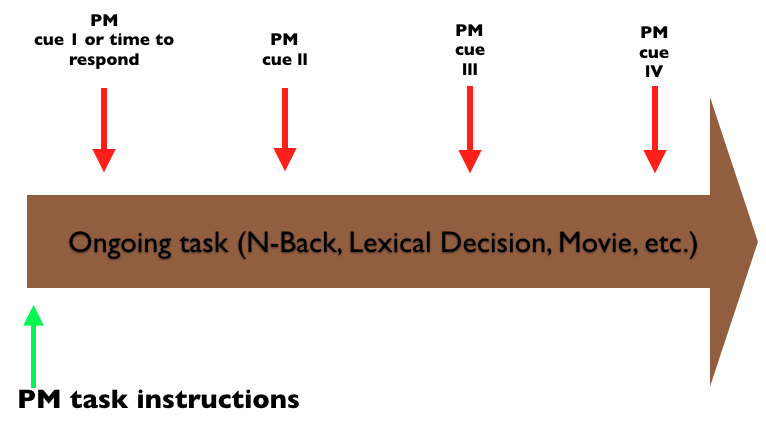
\includegraphics[width=10cm, height=6cm]{LAB.png} 
\centering
\end{frame}

%%%%%%%%%%%%%%%%%%%%%%%%%%%%%%%%%%%%%%%%%%%%%%%%%%%%%%
%%%%%%%%%%%%%%%%%%%%%%%%%%%%%%%%%%%%%%%%%%%%%%%%%%%%%%

\subsection{Valence and Prospective memory}
\begin{frame}{Two-dimensional model by valence and arousal}
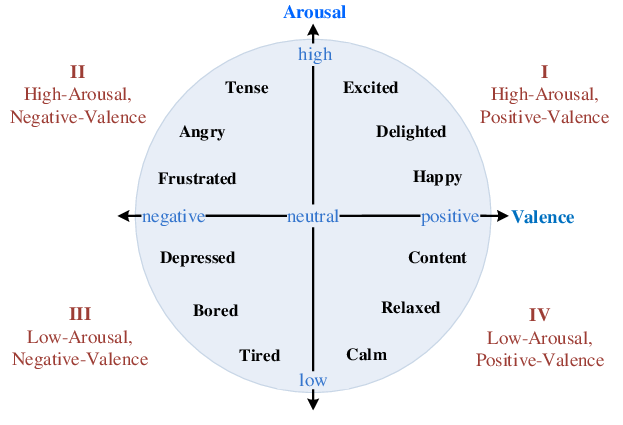
\includegraphics[scale=1.5]{Figure-1-Two-dimensional-valence-arousal-space.png} 
\centering
\end{frame}

%We remember only a fraction of life's experiences. While a multitude of factors can influence the likelihood that an event is remembered, one important contributor is the emotional salience of the event: events that contain emotional relevance are often more likely to be remembered than events devoid of emotional import. This memory-enhancing effect of emotion has been demonstrated in a large number of laboratory studies, using stimuli ranging from words to pictures to narrated slide shows (reviewed in 710,12,20,37/). Data from studies of autobiographical memory converge with the findings from the laboratory: individuals are more likely to remember personal experiences that contain some emotional salience 1221. Neuroimaging research and studies of brain lesioned patients have begun to clarify the neural processes contributing to memory for neutral and emotional experiences. In this review, I outline how these studies have begun to elucidate the effects that emotion has on the neural processes that allow us to remember information, focusing on the distinct effects exerted by valence and arousal (defined below) on declarative memory formation.

%To fully understand the ways in which emotion affects memory, it is important to recognize that emotional and neutral stimuli likely differ from one another in more than one dimension. A widely-accepted framework proposes that affective experiences are best characterized in a two-dimensional space (Fig. 1). The dimension of valence ranges from highly positive to highly negative, whereas the dimension of arousal ranges from calming or soothing to exciting or agitating 150,121. Thus, there can be events that are negative and agitating; positive and soothing; positive and exciting; etc.
%The majority of studies investigating declarative memory for emotional experiences have compared memory for neutral events (i.e., events that are neither highly positive nor highly negative; and that are not exciting or agitating) with events that are both arousing (i.e., exciting or agitating) and at an extreme on the valence dimension (either highly positive or highly negative). These studies leave unanswered the relative contributions of the valence dimension and the arousal dimension to the memory enhancement effect.

%Emotional arousal is clearly a critical factor contributing to the emotional enhancement effect for many types of information /16-18/. Nevertheless, there is evidence that memory can be enhanced even for positive or negative stimuli that do not elicit arousal (e.g., /44,63/). Further, there are reasons to believe that valence and arousal may contribute differently to memory formation and retrieval.

%Within perceptual domains, it is clear that valence and arousal (intensity) can have dissociable effects on the neural processes engaged during stimulus exposure. To distinguish the contributions of the arousal and valence dimensions on the neural response to odors, Anderson and colleagues /5/ independently manipulated odor valence (pleasant or unpleasant) and odor intensity. They found that amygdala activation was related to odor intensity irrespective of valence, whereas activity in the orbitofrontal cortex reflected valence regardless of intensity. Small and colleagues 1111 found a similar dissociation in the gustatory modality: the amygdala was responsive to taste intensity regardless of valence, whereas the orbitofrontal cortex was responsive to taste valence and but not to intensity.

%Recent research has suggested that a similar dissociation may exist with regard to the effects of valence and arousal on declarative, mnemonic processes. The amygdala may play a specific role in modulating memory for arousing events (see /16/ for an early proposal to this effect). As discussed below, the amygdala appears to influence the likelihood that the arousing information is processed (during encoding) and the likelihood that the encounter is preserved in a relatively stable memory trace (referred to as storage or consolidation). In contrast, although non-arousing events that are highly positive or highly negative can also be better remembered than neutral events, this enhancement may occur independently of amygdala activation.


%EMOTIONAL VALENCE AND ENCODING
%In comparison to the large number of studies investigating memory for arousing items, relatively few studies have examined memory for non-arousing positively or negatively valenced information. Nevertheless, the studies that have examined memory for these stimuli have suggested that the valence dimension is sufficient to boost memory performance. Thus, there are instances in which non-arousing items with positive or negative valence are better remembered than neutral ones /42,44,49,63/.
%
%The processes contributing to this enhancement, however, are likely distinct from those mediating the enhanced memory for arousing items. In contrast to the relatively automatic, attentional modulation discussed with regard to memory for arousing information, memory for non-arousing positive or negative stimuli may benefit instead from conscious encoding strategies, such as elaboration.

%Valence and elaboration
%
%Elaboration refers to the process of establishing links between newly encountered information and previously stored information. It has long been known that when individuals process items in an elaborative fashion, such that meaning is extracted from items and inter-item associations are formed, memory is enhanced /24,26,27/. A viable proposal is that, for positive and negative non-arousing stimuli, this ability to elaborate on the items is what leads to the enhanced memory. This elaborative processing could take at least two forms: auto- biographical and semantic.
%Autobiographical elaboration is known to benefit memory. For example, when individuals are asked to process stimuli in regard to themselves (e.g., deciding whether words would describe them), memory is enhanced as compared to when the items are processed for meaning, but not in relation to the self /54,71/. Thus, it is plausible that autobiographical elaboration may explain the memory benefit for non-arousing positive or negative items. It is reasonable that words such as 'sorrow' or 'comfort' may be more likely to be associated with autobiographical experiences or self-introspection than neutral words such as 'shadow'.
%Another possibility is that individuals are more likely to semantically elaborate on the valenced items - to think about the items' meanings, and their relationships to other items. Although this semantic elaboration could occur for a number of reasons, one possibility is that valenced items contain a semantic cohesiveness typically not present with neutral items. Consistent with this proposal, in at least some instances, the memory advantage for emotionally valenced items is reduced or eliminated when memory is compared for valenced words and neutral words with similar inter-item associations /49,80/.
%Numerous studies have shown that divided attention at encoding decreases a person's ability to carry out controlled encoding processes, such as autobiographical or semantic elaboration. There- fore, if these types of elaborative processes underlie the memory enhancement for non-arousing positive and negative items, then dividing people's attention as they encode these items should disrupt the memory advantage. This prediction has been upheld in a couple of studies showing that participants' memory for negative non-arousing words suffers with divided attention /13/ and that the memory advantage for negative, non-arousing words can be eliminated when participants encode items while simultaneously performing a secondary task /45/. These findings lend credence to the hypothesis that additional elaborative processing may underlie the memory enhancement at least for negative non-arousing words. Further research will need to be conducted to examine whether the same is true for positive non-arousing words.

%	\begin{itemize}
%	\item What is Valence?
%	\end{itemize}


%%%%%%%%%%%%%%%%%%%%%%%%%%%%%%%%%%%%%%%%%%%%%%%%%%%%%%
%%%%%%%%%%%%%%%%%%%%%%%%%%%%%%%%%%%%%%%%%%%%%%%%%%%%%%

\subsection{Three PM task aspects that can be influenced by valence}
\begin{frame}{Three PM aspects that can be influenced by valence}
  \begin{columns}[T]
    \begin{column}{.5\textwidth}
     \begin{block}{}
     \begin{itemize}
     	\item Cue
     	\item Intention
     	\item Context
     \end{itemize}
    \end{block}
    \end{column}
    \begin{column}{.5\textwidth}
    \begin{block}{}
% Your image included here
   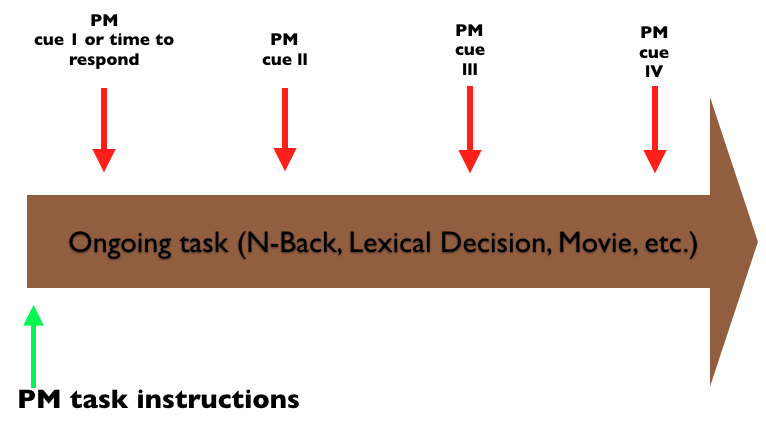
\includegraphics[width=6cm, height=5cm]{LAB.png} 
    \end{block}
    \end{column}
  \end{columns}
\end{frame}
%%%%%%%%%%%%%%%%%%%%%%%%%%%%%%%%%%%%%%%%%%%%%%%%%%%%%%
%%%%%%%%%%%%%%%%%%%%%%%%%%%%%%%%%%%%%%%%%%%%%%%%%%%%%%
 
%\subsubsection{Valenced Prospective Cue}
%\begin{frame}{Valenced Prospective Cue}
%	\begin{itemize}
%	\item More age differences in TBPM
%	\end{itemize}
%\end{frame}
%
%%%%%%%%%%%%%%%%%%%%%%%%%%%%%%%%%%%%%%%%%%%%%%%%%%%%%%%
%%%%%%%%%%%%%%%%%%%%%%%%%%%%%%%%%%%%%%%%%%%%%%%%%%%%%%%
%\subsubsection{Valenced Intention}
%\begin{frame}{Valenced Valenced Intention}
%	\begin{itemize}
%	\item More age differences in TBPM
%	\end{itemize}
%\end{frame}

%%%%%%%%%%%%%%%%%%%%%%%%%%%%%%%%%%%%%%%%%%%%%%%%%%%%%%
%%%%%%%%%%%%%%%%%%%%%%%%%%%%%%%%%%%%%%%%%%%%%%%%%%%%%%

%\subsubsection{Valenced Context}
%\begin{frame}{Valenced Context}
%\end{frame}


%%%%%%%%%%%%%%%%%%%%%%%%%%%%%%%%%%%%%%%%%%%%%%%%%%%%%%
%%%%%%%%%%%%%%%%%%%%%%%%%%%%%%%%%%%%%%%%%%%%%%%%%%%%%%


%\subsection{TBPM and Time Estimation}
%\begin{frame}{TBPM and Time Estimation}
%\begin{figure}[hbtp]
%\centering
%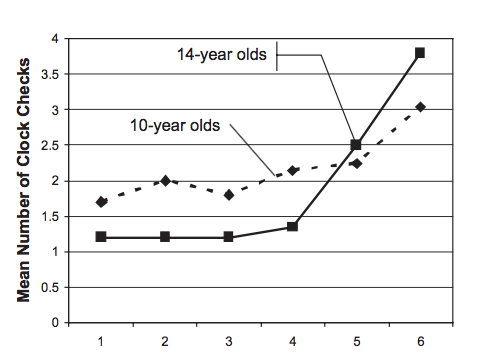
\includegraphics[width=10cm, height=6cm]{PM.png}
%\caption{Ceci, S. J., \& Bronfenbrenner, U. (1985)}
%\end{figure}
%
%\end{frame}


%%%%%%%%%%%%%%%%%%%%%%%%%%%%%%%%%%%%%%%%%%%%%%%%%%%%%%
%%%%%%%%%%%%%%%%%%%%%%%%%%%%%%%%%%%%%%%%%%%%%%%%%%%%%%
%\subsection{Emotional Influences on Time Estimation}
%\begin{frame}{Emotional influences on time estimation}
%\begin{figure}[hbtp]
%\centering
%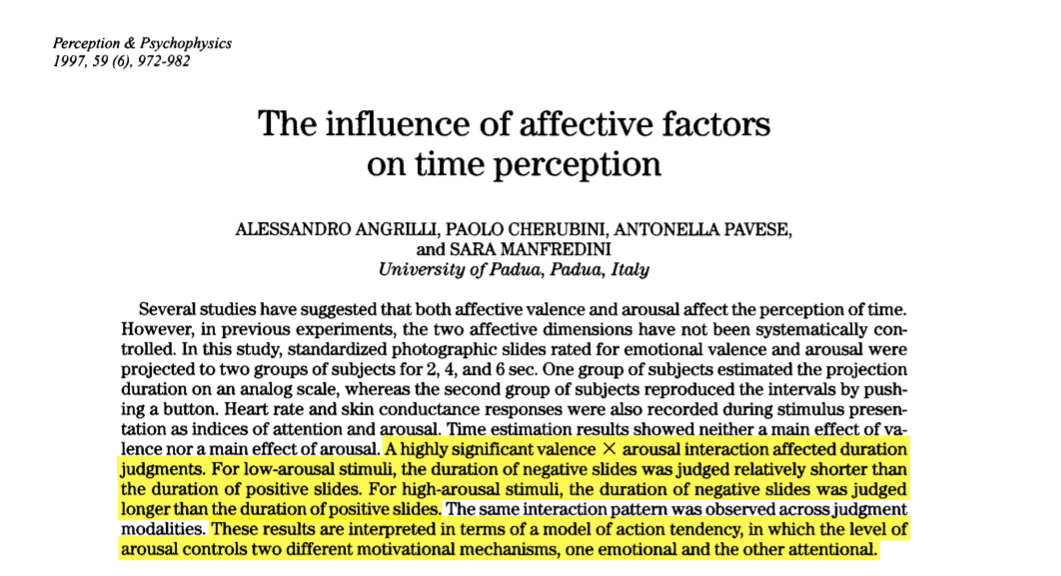
\includegraphics[width=10cm, height=6cm]{ANGRI.png}
%\end{figure}
%\end{frame}

%%%%%%%%%%%%%%%%%%%%%%%%%%%%%%%%%%%%%%%%%%%%%%%%%%%%%%
%%%%%%%%%%%%%%%%%%%%%%%%%%%%%%%%%%%%%%%%%%%%%%%%%%%%%%
\section{\scshape Methodology}
\subsection{Aim}
\begin{frame}{Aim}
\begin{itemize}
\item Problem:
\begin{itemize}
\item Does ongoing activity stimuli affective valence affects TBPM performance even if arousal is maintained constant?

\item Are there context valence X age interactions in PM performance, clock monitoring and/or ongoing activity performance?

\item Are there any theoretical model that can explain obtained results?
\end{itemize}

\item Justification: To our knowledge, age x context valence effects has not yet been the focus of a systematic investigation in the context of a TMPM task.
\end{itemize}
\end{frame}


%%%%%%%%%%%%%%%%%%%%%%%%%%%%%%%%%%%%%%%%%%%%%%%%%%%%%%
%%%%%%%%%%%%%%%%%%%%%%%%%%%%%%%%%%%%%%%%%%%%%%%%%%%%%%

\subsection{Participants}
\begin{frame}{Participants}
\begin{itemize}
\item Participants: 20 Young adults (18-25 years) \& 20 Old adults (60-75 years). Years of schooling 12 years.
\item Neuropsychological Batteries:
	\begin{itemize}
	\item Depression Anxiety and Stress Scale (DASS-21) 
	\item Psychological Battery for Attention Assessment (BPA)- (Rueda, 2013)
	\item The Cambridge Cognitive Examination-Revised (CAMCOG-R)
	\end{itemize}
%\item Physiological measures
%	\begin{itemize} 
%	\item Skin Conductance Responses (SCRs)
%	\item Hearth Rate
%	\item Eye tracking
%	\end{itemize}
\item Laboratory tasks: Time reproduction \& TBPM
\end{itemize}
\end{frame}

%%%%%%%%%%%%%%%%%%%%%%%%%%%%%%%%%%%%%%%%%%%%%%%%%%%%%%
%%%%%%%%%%%%%%%%%%%%%%%%%%%%%%%%%%%%%%%%%%%%%%%%%%%%%%

\subsection{Time Based Prospective Memory Task}
\begin{frame}{Time Based Prospective Memory Task}
  \begin{columns}[T]
    \begin{column}{.5\textwidth}
     \begin{block}{}
     \begin{itemize}
     \item Three Conditions:
     \begin{itemize}
     \item Positive Valence IAPS
     \item Negative Valence IAPS
     \item Neutral Valence IAPS
     \end{itemize}
     \item Ongoing Activity Performance (Acurracy and RT)
     \item Clock Monitoring Performance
     \item Prospective Memory Performance (Acurracy 5s before or after the required response time)
     %\item Physiological measures
     \end{itemize}
    \end{block}
    \end{column}
    \begin{column}{.5\textwidth}
    \begin{block}{}
% Your image included here
    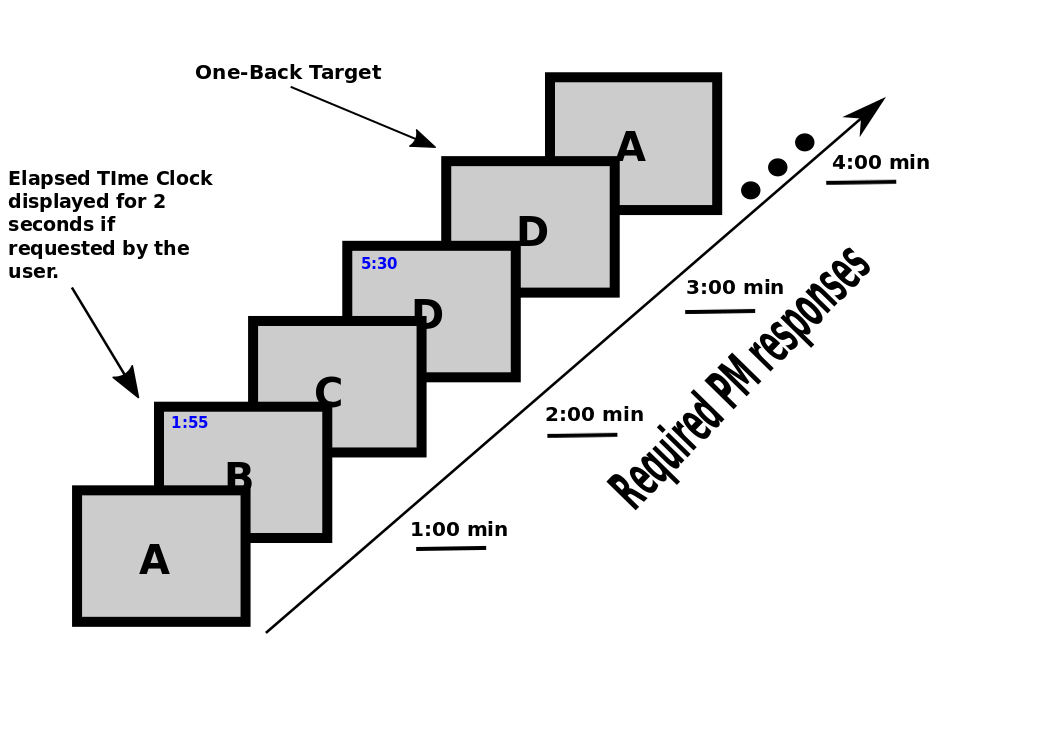
\includegraphics[width=6.5cm, height=7cm]{Oneback.png}
    \end{block}
    \end{column}
  \end{columns}
\end{frame}


%%%%%%%%%%%%%%%%%%%%%%%%%%%%%%%%%%%%%%%%%%%%%%%%%%%%%%
%%%%%%%%%%%%%%%%%%%%%%%%%%%%%%%%%%%%%%%%%%%%%%%%%%%%%%
%\subsection{Time Reproduction Task}
%\begin{frame}{Time Reproduction Task}
%  \begin{columns}[T]
%    \begin{column}{.5\textwidth}
%     \begin{block}{}
%          \begin{itemize}
%     \item Random Stimuli:
%     \begin{itemize}
%     \item Positive Valence IAPS
%     \item Negative Valence IAPS
%     \item Neutral IAPS
%     \end{itemize}
%     \item Time Reproduction Performance
%     \item Physiological measures
%     \end{itemize}
%    \end{block}
%    \end{column}
%    \begin{column}{.5\textwidth}
%    \begin{block}{}
%% Your image included here
%    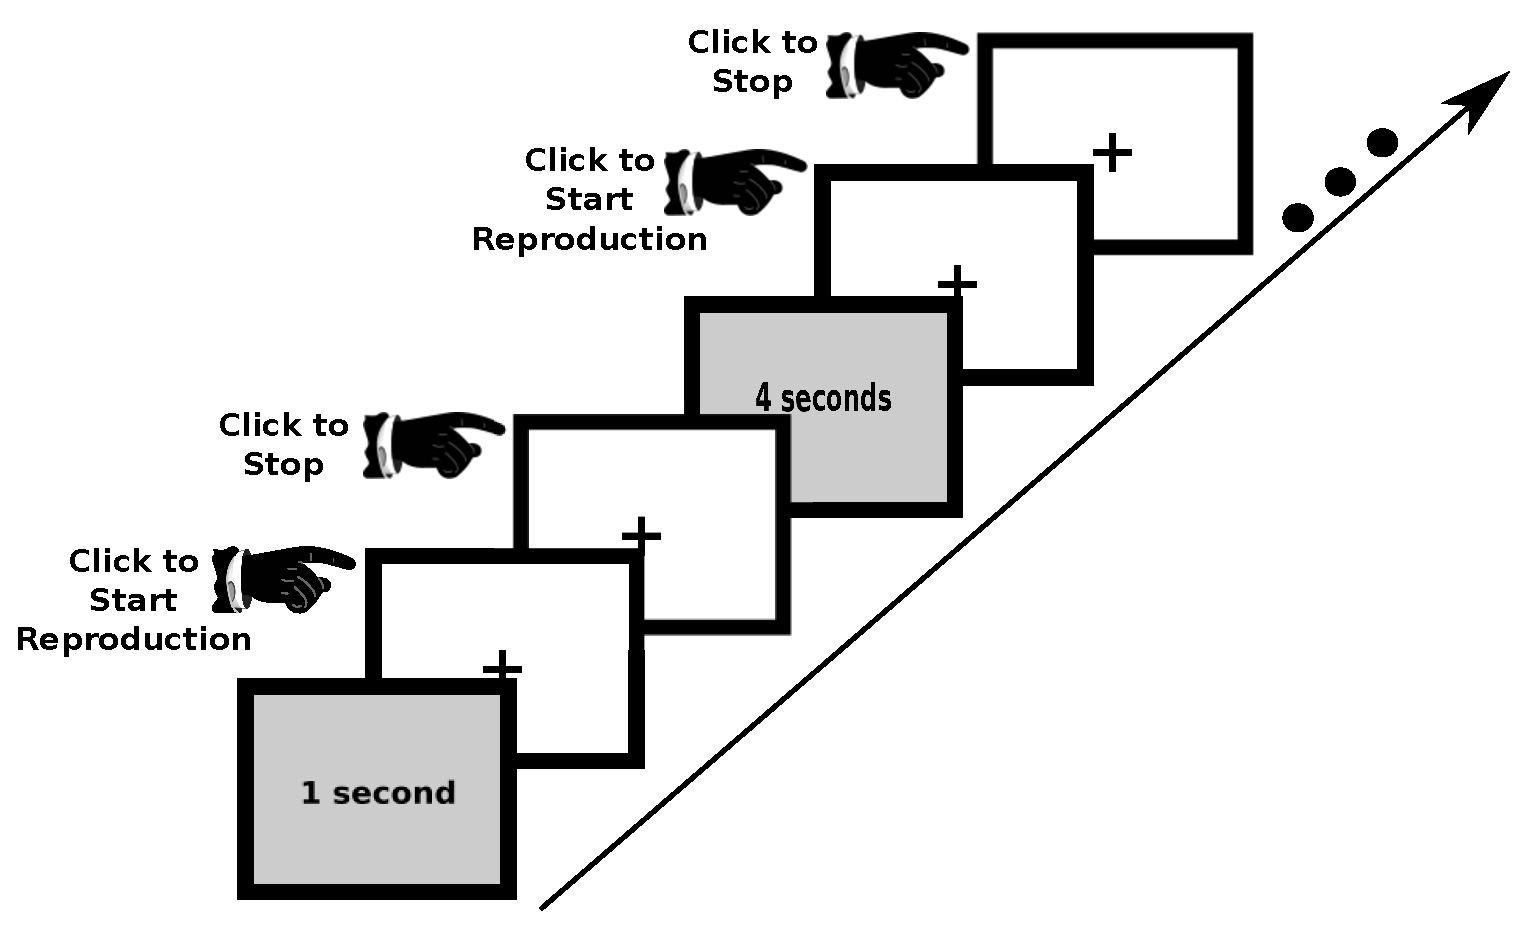
\includegraphics[width=6cm, height=6cm]{timerepro.eps} 
%    \end{block}
%    \end{column}
%  \end{columns}

%\end{frame}

%%%%%%%%%%%%%%%%%%%%%%%%%%%%%%%%%%%%%%%%%%%%%%%%%%%%%%
%%%%%%%%%%%%%%%%%%%%%%%%%%%%%%%%%%%%%%%%%%%%%%%%%%%%%%

\section{\scshape Looking Forward}
\begin{frame}{Looking Forward}
\begin{itemize}
	\item October
		\begin{itemize}
			\item Completion of Experiments and Early Analysis 
		\end{itemize}
	\item November
		\begin{itemize}
			\item Analysis and Manuscript Preparation
		\end{itemize}
	\item December
		\begin{itemize}
			\item Manuscript Preparation and Dissertation Preparation
		\end{itemize}
	\item January 2018
		\begin{itemize}
			\item Paper Submission and Dissertation Preparation
		\end{itemize}
	\item February 2018
		\begin{itemize}
			\item Master's Defense
		\end{itemize}
\end{itemize}

\end{frame}


%%%%%%%%%%%%%%%%%%%%%%%%%%%%%%%%%%%%%%%%%%%%%%%%%%%%%%
%%%%%%%%%%%%%%%%%%%%%%%%%%%%%%%%%%%%%%%%%%%%%%%%%%%%%%
\section{\scshape References}
\begin{frame}{References}
\begin{itemize}
\begin{tiny}
\item Altgassen, M., Phillips, L. H., Henry, J. D., Rendell, P. G., \& Kliegel, M. (2010). Emotional target cues eliminate age differences in prospective memory. Quarterly Journal of Experimental Psychology (2006), 63(6), 1057– 64.
\item Angrilli, A., Cherubini, P., Pavese, A., \& Mantredini, S. (1997). The influence of affective factors on time perception. Perception \& Psychophysics, 59(6), 972–82.
\item Block, R. A., \& Zakay, D. (2006). Prospective Remembering Involves Time Estimation and Memory Processes. In Timing the future: The case for a time-based prospective memory. (pp. 25–49).
\item Einstein, G. O., \& McDaniel, M. a. (2005). Prospective Memory Multiple Retrieval Processes. Current Directions in Psychological Science, 14(6), 286.
\item Henry, J. D., MacLeod, M. S., Phillips, L. H. and Crawford, J. R. (2004). A metaanalytic review of prospective memory and aging. Psychology and Aging, 19, 27–39.
\item Huppert, F. A., Johnson, T. and Nickson, J. (2000). High prevalence of prospective memory impairment in the elderly and in early-stage dementia: findings from a population based study. Applied Cognitive Psychology, 14, S63–S81.
\item Lake, J. I. (2015). Emotional modulation of time perception. Dissertation Abstracts International: Section B: The Sciences and Engineering, 76(1–B(E)), No-Specified.
\item Rendell, P. G. and Thomson, D. M. (1999). Aging and prospective memory: differences between naturalistic and laboratory tasks. The Journals of Gerontology: Psychological Sciences, 54B, 256–269.
\item Schnitzspahn, K. M., Ihle, A., Henry, J. D., Rendell, P. G., \& Kliegel, M. (2011). The age-prospective memory- paradox: an exploration of possible mechanisms. International Psychogeriatrics , IPA, 23(4), 583–592.
\item Schnitzspahn, K. M., Thorley, C., Phillips, L., Voigt, B., Threadgold, E., Hammond, E. R., ... Kliegel, M. (2014). Mood impairs time-based prospective memory in young but not older adults: The mediating role of attentional control. Psychology and Aging, 29(2), 264–70.
\item Waldum, E. R., \& McDaniel, M. A. (2016). Why are you late? Investigating the role of time management in time- based prospective memory. Journal of Experimental Psychology: General, 145(8), 1049–1061.
\end{tiny}
\end{itemize}
\end{frame}


\end{document}